\documentclass[border=10pt]{standalone}
\usepackage{circuitikz}
\usepackage{tikz}
\usetikzlibrary{calc, positioning, arrows.meta, shapes.geometric}

\begin{document}
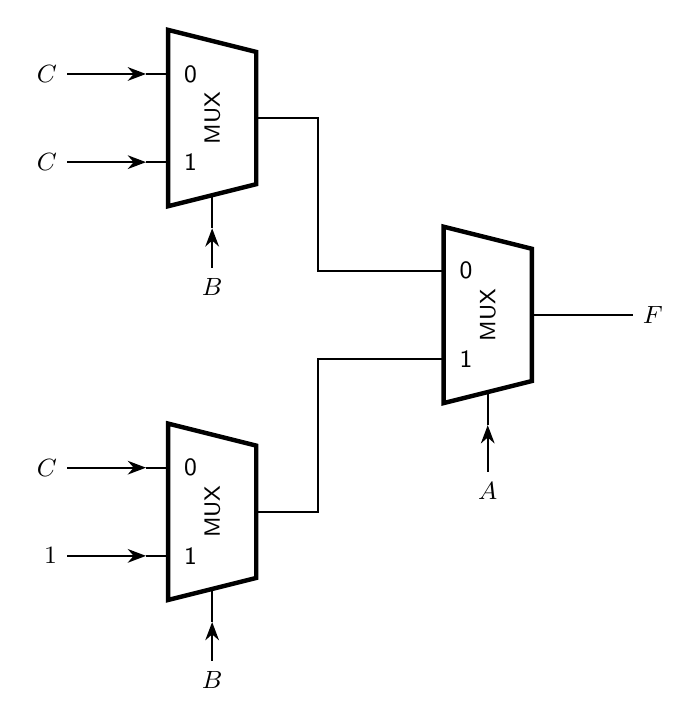
\begin{tikzpicture}[
    >=Stealth, 
    thick, 
    font=\sffamily\small
]

    % Global style for standard mux
    \tikzset{
        stdmux/.style={
            muxdemux, 
            muxdemux def={Lh=4, NL=2, Rh=3, NB=1, w=2.0, NT=0, square pins=1}
        }
    }

    % Level 1 MUX (A)
    \node[stdmux] (M1) at (0, 0) {\rotatebox{90}{\footnotesize MUX}};
    
    % M1 Output
    \draw (M1.rpin 1) -- ++(1, 0) node[right] {$F$}; 

    % M1 Select (A)
    \draw[<-] (M1.bpin 1) -- ++(0, -0.6) node[below] {$A$}; 

    % M1 Inputs Labels
    \node[right][xshift=1em] at (M1.lpin 1) {0};
    \node[right][xshift=1em] at (M1.lpin 2) {1};

    % Level 2 MUXs (B)
    \node[stdmux] (M2_0) at (-3.5, 2.5) {\rotatebox{90}{\footnotesize MUX}}; 
    \draw[<-] (M2_0.bpin 1) -- ++(0, -0.5) node[below] {$B$}; % Select B
    
    \node[stdmux] (M2_1) at (-3.5, -2.5) {\rotatebox{90}{\footnotesize MUX}}; 
    \draw[<-] (M2_1.bpin 1) -- ++(0, -0.5) node[below] {$B$}; % Select B

    % Wiring M2 -> M1
    % M2_0 Output -> M1 Input 0 (lpin 1)
    \draw (M2_0.rpin 1) -- ++(0.5, 0) |- (M1.lpin 1);
    
    % M2_1 Output -> M1 Input 1 (lpin 2)
    \draw (M2_1.rpin 1) -- ++(0.5, 0) |- (M1.lpin 2);
    
    % M2 Inputs Labels
    \node[right][xshift=1em] at (M2_0.lpin 1) {0};
    \node[right][xshift=1em] at (M2_0.lpin 2) {1};

    \node[right][xshift=1em] at (M2_1.lpin 1) {0};
    \node[right][xshift=1em] at (M2_1.lpin 2) {1};

    % Wiring Inputs
    \draw[<-] (M2_0.lpin 1) -- ++(-1, 0) node[left] {$C$};
    \draw[<-] (M2_0.lpin 2) -- ++(-1, 0) node[left] {$C$};
    
    \draw[<-] (M2_1.lpin 1) -- ++(-1, 0) node[left] {$C$};
    \draw[<-] (M2_1.lpin 2) -- ++(-1, 0) node[left] {$1$};

    % Labels
  %  \node[above, blue] at (-2, 4) {Co-factors of A};
  %  \node[above, blue] at (-5.5, 4) {Co-factors of B};

\end{tikzpicture}
\end{document}
